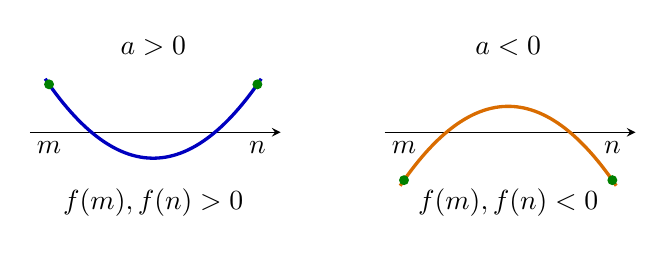
\begin{tikzpicture}[x=.98cm,y=.83cm,>=stealth]
 \begin{scope}[shift={(-2.3,0)}]
  \draw[->] (-1.6,0)--(1.65,0);\draw[very thick,blue!75!black,domain=-1.4:1.4,samples=60] plot (\x,{.62*(\x*\x-.64)});
  \node[above] at (0,1.02) {$a>0$};\node[below] at (-1.35,0) {$m$};\node[below] at (1.35,0) {$n$};
  \fill[green!50!black] (-1.35,{.62*(1.35*1.35-.64)}) circle(1.8pt) (1.35,{.62*(1.35*1.35-.64)}) circle(1.8pt);
  \node[below] at (0,-.72) {$f(m),f(n)>0$};
 \end{scope}
 \begin{scope}[shift={(2.3,0)}]
  \draw[->] (-1.6,0)--(1.65,0);\draw[very thick,orange!85!black,domain=-1.4:1.4,samples=60] plot (\x,{-.62*(\x*\x-.64)});
  \node[above] at (0,1.02) {$a<0$};\node[below] at (-1.35,0) {$m$};\node[below] at (1.35,0) {$n$};
  \fill[green!50!black] (-1.35,{-.62*(1.35*1.35-.64)}) circle(1.8pt) (1.35,{-.62*(1.35*1.35-.64)}) circle(1.8pt);
  \node[below] at (0,-.72) {$f(m),f(n)<0$};
 \end{scope}
\end{tikzpicture}
